% Chapitre 17 -- G-RUSTY : rusty-SUNDIALS, traduction en Rust du solveur CVODE assistée par IA
% Sources : results/discovery_journal_2026/TOP20.json (pick 17) ; github_inventory.md (rusty-SUNDIALS) ;
% rusty-SUNDIALS main, docs/audit/fusion-2026-09-27/{RETRACTION_NOTICE.md,B_numerics.md} et README.md (lus via gh api le 26/10/2026) ;
% .zenodo.json du dépôt (même date) ; papers/prog_population_genetics_fixation/AUDIT.md et papers/ar_sigma3_enstrophy/AUDIT.md
% (réexécutions identiques) ; mémoire fusion-project-audit.md et openai-math-crosswalk.md. Figure : code/fig17.py.
\chapter[Le moteur des calculs]{Le moteur des calculs, et son rapport d'inspection}
\reference{Dépôt public créé le 11 mai 2026. Audit et rétractations fusionnés le 27 septembre 2026 (demande de fusion n\textsuperscript{o}~60). Pas de DOI propre.}

\noindent\niveau{X} pour tout ce que le solveur calcule~: ce sont des nombres en virgule flottante, ils guident et
ne prouvent jamais.

\section*{L'idée en une image}

\begin{analogie}
Vous réglez une douche dont l'eau réagit vite. La méthode naïve consiste à regarder la température \emph{maintenant}
et à tourner le robinet d'autant~: si vous tournez trop fort, l'eau passe de trop chaude à trop froide, puis à
encore plus chaude, et l'écart grandit à chaque correction. La méthode prudente consiste à choisir la position du
robinet qui sera juste \emph{une fois la correction faite}. Elle demande un petit calcul à chaque geste, mais elle ne
s'emballe jamais. Les équations dites \og raides\fg, où certaines choses changent beaucoup plus vite que d'autres,
sont des douches de ce genre~; le solveur CVODE est construit pour elles.

\emph{Où l'image cesse d'être juste~:} un solveur ne \og sent\fg{} rien, il résout une équation à chaque pas~; et la
méthode prudente reste stable sans être forcément précise, comme on le voit ci-dessous.
\end{analogie}

\section*{Ce qui a été fait}

SUNDIALS est une bibliothèque de calcul scientifique très utilisée, écrite en langage C par un laboratoire national
américain~; CVODE en est la partie qui résout les équations raides de la chimie, des plasmas ou de la biologie.
Dès le 11 mai 2026, des agents d'IA, sous la direction de l'auteur, en ont fait une traduction en langage Rust,
rusty-SUNDIALS. C'est devenu l'instrument de l'année~: les distances cosmologiques du chapitre~1, les probabilités
de fixation du chapitre~7, plusieurs des contributions du 25 octobre et d'autres articles s'appuient sur ses calculs.

\paragraph{Un exemple à suivre au crayon.} Prenez l'équation $y'=-50\,y$ avec $y(0)=1$, et un pas de temps $h=0{,}05$.
La vraie solution est multipliée par $e^{-2{,}5}\approx0{,}082$ à chaque pas~: elle s'éteint très vite.
\begin{itemize}
\item La méthode naïve (Euler explicite) calcule $y_{n+1}=y_n+h\times(-50\,y_n)=(1-2{,}5)\,y_n=-1{,}5\,y_n$~:
  $1$, puis $-1{,}5$, puis $2{,}25$, puis $-3{,}375$\ldots{} Elle explose en changeant de signe, comme la douche.
\item La méthode prudente (Euler implicite) impose $y_{n+1}=y_n-2{,}5\,y_{n+1}$, donc $y_{n+1}=y_n/3{,}5$~:
  $1$, $0{,}286$, $0{,}082$\ldots{} Moins précise que la vraie solution à chaque pas, mais toujours sage.
\end{itemize}
La naïve ne marche que si $50\,h<2$, c'est-à-dire $h<0{,}04$. La figure~\ref{fig:c17} montre ce seuil sur une
équation voisine. Ce calcul est fait en Python pour ce livre~: il illustre le phénomène, ce n'est pas une sortie de
rusty-SUNDIALS.

\section*{Comment on s'est assuré que ce n'est pas faux}

Il faut séparer deux choses~: les résultats des articles qui utilisent le solveur, et ce que le dépôt affirmait de
lui-même.

Pour les articles de l'automne, des auditeurs (des agents d'IA distincts des producteurs) ont relancé les calculs
CVODE et obtenu des fichiers identiques octet pour octet à ceux publiés. Cela prouve que le calcul est
reproductible, pas qu'il est juste~; c'est pourquoi ces nombres restent au niveau~X et que les articles ne
s'appuient sur eux pour aucune affirmation démontrée.

Pour le dépôt lui-même, l'histoire est moins flatteuse, et elle compte autant. Le 27 septembre, trois agents d'IA
séparés ont audité ses travaux sur la fusion (les disruptions du réacteur ITER)~: l'un a relu les affirmations des
articles, un autre a relancé les calculs, un troisième a vérifié les fichiers Lean. Leur constat~:
\begin{itemize}
\item des nombres publiés n'étaient produits par aucun code du dépôt~; c'étaient des valeurs tapées à la main~;
\item un programme affichait \og accélération de 47 fois mathématiquement vérifiée\fg~; sans les pauses
  (\texttt{sleep}) insérées dans le code, le rapport des deux temps valait $1{,}00$~;
\item le tracé d'une formule fixée d'avance passait pour une \og simulation\fg{} de plasma~;
\item des \og certificats\fg{} Lean étaient vides, ou reposaient sur des axiomes dont on peut déduire le faux,
  ce que l'audit a démontré dans le noyau lui-même.
\end{itemize}
Une notice de rétractation a été fusionnée le jour même. Rien n'a été effacé~: chaque document porte un bandeau qui
renvoie à la notice, et le code qui imprimait des verdicts inventés affiche désormais ce qu'il mesure, ou \og NON
MESURÉ\fg. Sur ses propres tests de contrôle, l'audit a trouvé le solveur correct aux tolérances modérées, et il a
noté qu'un cas plus raide échoue à tolérance très fine. Aucun humain n'a relu ces audits.

\section*{Ce que ça ne dit pas}

\begin{limite}
\begin{itemize}
\item Le solveur n'est pas \og formellement vérifié\fg, malgré ce qu'annonce encore la première page de son dépôt.
  Ses sorties sont des calculs en virgule flottante (\niveau{X}).
\item Plusieurs fichiers de spécification Lean du dépôt contiennent des axiomes vides ou incohérents~; il ne faut
  rien construire dessus.
\item Au 26 octobre 2026, la fiche de métadonnées du dépôt reprend encore des affirmations rétractées~; l'audit a
  laissé ce choix au propriétaire, et il n'est pas fait.
\item Un fichier identique octet pour octet montre que le calcul se refait, pas qu'il est exact.
\item L'audit a relevé une différence avec l'original dans la réaction du solveur à des échecs répétés de son
  test d'erreur~; il la signale comme hypothèse, non vérifiée.
\end{itemize}
\end{limite}

\section*{Pour aller plus loin}

Le dépôt public rusty-SUNDIALS contient le code, et le dossier de l'audit du 27 septembre (notice de rétractation
et trois rapports). Le chapitre~20 raconte une autre méthode numérique accusée à tort, puis mesurée.

\begin{figure}[t]
\centering
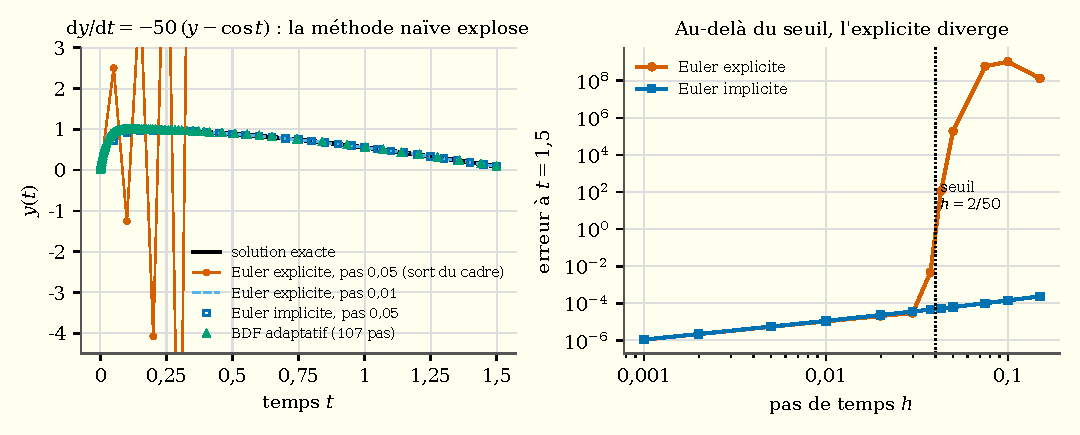
\includegraphics[width=\linewidth]{figures/c17_raideur}
\caption{Calcul d'illustration en Python (pas rusty-SUNDIALS). À gauche~: l'équation raide $y'=-50(y-\cos t)$~; la
méthode naïve au pas $0{,}05$ explose, les autres suivent la solution exacte. À droite~: erreur finale selon le pas~;
la naïve diverge au-delà de $h=2/50$.}
\label{fig:c17}
\end{figure}
